\documentclass{article}
\usepackage[utf8]{inputenc}
\usepackage{multicol}
\usepackage{Preamble}
\usepackage{subfiles}


\title{Do Globular Clusters contain Intermediate-Mass Black Holes?}
\author{Bobby Hemming}
\date{March 2018}

\begin{document}
\maketitle
\begin{abstract}
Abstract Abstract Abstract Abstract Abstract Abstract Abstract Abstract Abstract Abstract Abstract Abstract Abstract Abstract Abstract Abstract Abstract Abstract Abstract Abstract Abstract Abstract Abstract Abstract Abstract Abstract Abstract Abstract Abstract Abstract Abstract Abstract Abstract Abstract 
\end{abstract}
\begin{multicols}{2}



\section{Introduction}

\subsection{Background}
Globular Clusters (GCs) are some of the oldest astronomical structures in the Universe, having formed 1 to 2 Gyrs after the big bang. Research into their evolution can provide an insight into  the early universe. GCs are spherical collections of stars that orbit a galactic core and are tightly bound by gravitational forces. The Milky Way (MW) has around 150 “satellite” GCs that are ~$10^4$ solar masses (M$_{\odot}$) and orbit the core at radii of up to 40 kiloparsecs (130,000 light-years). GCs are extremely luminous objects, approximately $25,000$ times as luminous as the sun (L$_{\odot}$), despite 90$\%$ of the mass made up from fainter stars. 

The origin of GCs is still poorly understood, but most show stars in the same stage of evolution, suggesting they were formed about the same age. As the GCs evolve the stars exchange energy in two-body interactions; stars with low energy are found in the centre of the cluster, they sink to the bottom of the potential well. This is dynamic relaxation also known as core collapse and is caused by gravitational instability in the core. This work will aim to investigate core collapse, as explained in section 1.3. The composition of GCs is mainly of population II star, with a large concentration at the core and fewer, further out in a more diffuse halo. They contain a low proportion of elements other than hydrogen and helium.

A topical question regarding GCs is if they contain Intermediate-Mass black holes (IMBHs) ~$100$ to $10^5$ M$_{\odot}$. There is strong evidence for stellar mass black holes ~$10$ to $100$ M$_{\odot}$ and for super-massive black holes (SMBHs) ~$10^5$ to $10^9$ M$_{\odot}$ at galactic cores; in the case of the MW the SMBH location corresponds to that of Sagittarius A$^*$, a bright radio-source at the centre. There is no conclusive evidence for IMBHs, however it’s believed they could exist at the centre of GCs, but is still a very hypothetical line of research. 

Current work investigating black holes at the centre of GCs comes from radial velocity measurements of stars orbiting the core to see if they have unusually high velocities. This research aims to probe Globular Cluster collapse and the effect that IMBHs have on the cluster.


\subsection{Theory}
The most important factor to consider in an astronomical system such as a GC is gravity. Gravitational forces dominate over large distances and are always attractive, so bodies will always accelerate towards each other. 
\begin{equation}
    \textbf{F}_{i} = -G \sum_i^N m_i m_j \frac{\textbf{r}_i - \textbf{r}_j} {[|r_i-r_j|^2]^\frac{3}{2}}
    \label{F}
\end{equation}
As seen in Eqn.(\ref{F}) the force on a body, $\textbf{F}_{i}$ in a GC depends only on the location of a body relative to all the other bodies. The labels m$_i$, m$_j$ are the masses of two bodies modelled as point masses, $G$ is the gravitational constant, $|r_i - r_j|$ is the separation of the bodies and $\textbf{r}_i$, $\textbf{r}_j$ are the position vectors.

The Virial theorem states that for a stable, self gravitating, spherical system of equal mass objects, the total kinetic energy is equal to negative a half of the total potential energy \cite{Virialreference}. This means for a stable GC (no dynamic relaxation) the total potential and kinetic energy of the GC should follow Eqn.(\ref{V}),
\begin{equation}
    2T + V = 0  
    \label{Virial}
\end{equation}
where the total kinetic energy is given my $T$, detailed by  Eqn.(\ref{T}) for a GC and 
\begin{equation}
    T = \frac{1}{2} \sum_{i=1}^{N} m_i v_i^2  
    \label{T}
\end{equation}
the total potential is given by $V$, detailed by  Eqn.(\ref{T}) for a GC.
\begin{equation}
     V = -\frac{G}{2} \sum_{i=1}^{N} \sum_{j=1}^{N}\frac{m_i m_j}{|r_i-r_j|^2}   
    \label{V}
\end{equation}
The labels in Eqn.(\ref{T}) and Eqn.(\ref{V}) are the same as before and with $v_i$ referring to the speed of each particle in the cluster. Both equations sum over all the particles in the cluster to get the total kinetic and potential.

An assumption of the Virial theorem is that all of the orbits travel on similar orbits that are isotropic, that is that they do not have any preferred direction. The Virial theorem can be rearranged to give the Virial mass, $M_{tot}$:
\begin{equation}
    M_{tot} \simeq 2\frac{R_{tot} v^2}{G}
    \label{Virial2}
\end{equation}
where the mass has been summed over all the particles to give $M_{tot}$, $R_{tot}$ is the total radius of the cluster and $v$ is the radial velocity of the cluster which can be found by measuring the velocity dispersion ($v^2 = 3\sigma_D^2$ in 3 dimensions).
By rearranging Eqn.(\ref{Virial2}) for $v$ and the defining the crossing time, $t_{cr}$ as the average time taken for a particle to cross over the whole cluster ($t_{cr}$=$2R$/$v$) then we have,
\begin{equation}
    t_{cr} \approx \frac{1}{\sqrt{G\rho_c}}
    \label{crossingtime}
\end{equation}
where $\rho_c$ is the density of the cluster. An interesting point to note is that it's expected, as in a gas, that as a GC evolves it should move to a state of higher entropy.  If we take a body in the GC and remove energy from it, it will descend to a lower orbit. The Virial theorem tells us that the decrease in potential energy is twice as big as the increase in kinetic energy, therefore we have net removal of energy from the system. Furthermore, energy has been removed, but the temperature of the system has increased ($v$ has increased), therefore GCs are said to have a negative specific heat.

% Since GCs have a finite mass, they have a finite escape velocity, so sometimes stars have enough energy to remove themselves from the cluster. Maybe a bit on this?

Velocity Dispersion Profiles????!!!

\subsection{Aims}

This research aims to investigate the effect of IMBHs on GC evolution. Principally it will test the quantities described in section 1.2, such as potential and kinetic energy, velocity dispersion's and root mean square radii of the cluster of certain GCs to identify the key differences between a cluster with an IMBH and one without. The aim is to use a computational approach (see section 3) as the N-body problem is to complex to solve analytically; each bodies contribution must be counted as it effects the overall system. Several different spherical GCs will be simulated with different initial conditions (detailed in section 3.2) for different $M_{IMBH}$/$M_{GC}$ (IMBH GC mass fractions), initial concentrations and sizes. 


\section{Past Work}

\subsection{History}
The first cluster to be observed was Messier 22 (M22), discovered in 1665 by Abraham Isle, a German amateur astronomer, but because of early telescope's small apetures, stars were not resolved in clusters until Charles Messier observed Messier 4 (M4) in 1764 \cite{GCorigins}. Since then, simulating GCs has been an important advance in research in this area as it allows astronomers to follow a GC evolution over millions of years and for many more stars than is possible observationally or analytically. Important milestones in GC simulations are by Sparzem & Aarseth 1996 ($10^4$ stars), Baumgardt and Makino 2003 ($10^5$ stars) \cite{HB} and Long Wang et al. 2016 ($10^6$ stars) \cite{LW}.   

\subsection{Dr H. Baumgardt}
Work by Dr H. Baumgardt is relevant to my work as part of his work concludes the possibility of an IMBH at the centre of Omega Centauri ($\omega$ Cen), the largest GC in the MW \cite{HB}. Initially Baumgardt sets out to determine the mass to light ratio of GCs by comparing real data collected by Karl Gebhardt et al. for the velocity dispersion and surface brightness profiles of $\omega$ Cen against his simulations using the N-body code NBODY6 for clusters with and without IMBHs. The models follow 900 N-body star clusters and varies the initial concentration, size and black hole mass. The model also incorporates the effects of stellar evolution and mass segregation. The simulation was run with N $=$ 100,000 stars, IMBH mass $\approx$ 40,000 M$_{\odot}$ allowed to evolve for up to 13.5 Gyrs.
\vspace{4mm}
    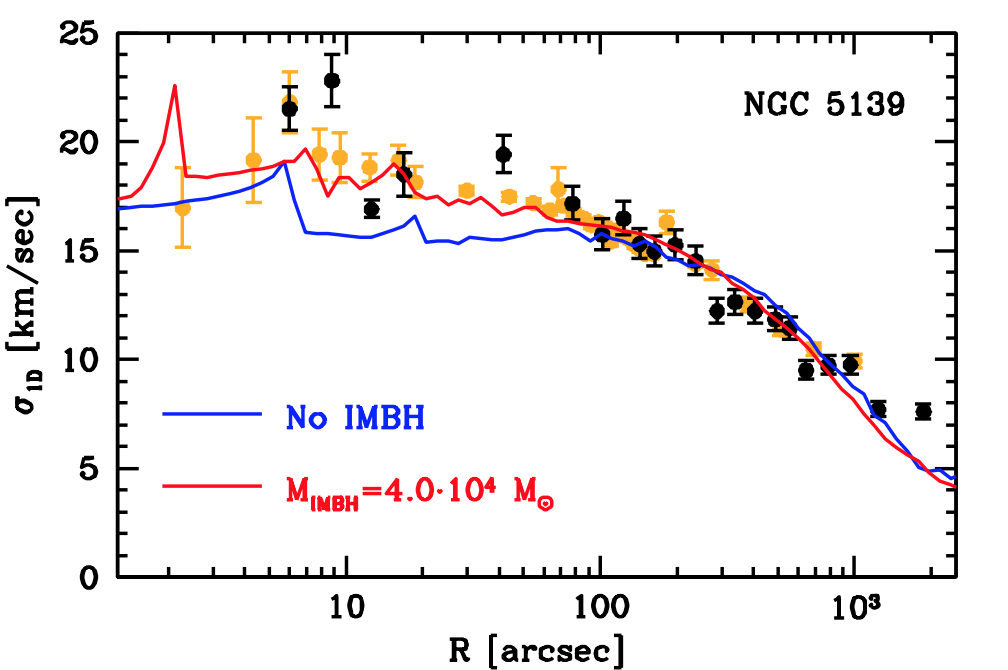
\includegraphics[width=0.45\textwidth]{HB.PNG}
    
    
    \captionof{\textbf{Figure 1.}} {\small Velocity dispersion profile of $\omega$ Cen taken from Fig. 6 of the work by Dr H. Baumgardt \cite{HB} which shows the strongest evidence for the presence of an IMBH in a GC. The red line shows the simulation containing an IMBH and the blue line shows the simulation with no IMBH, both are plotted against observed data for the cluster.}
\vspace{2mm}

It can clearly be seen from Fig.1 that the velocity dispersion profile for $\omega$ Cen without a IMBH is in strong disagreement with the observed data. Baumgardt reports a value for $\chi^2$ = 2.71, his second largest disagreement with the observed data. Therefore, his research suggests $\omega$ Cen contains an IMBH. This is an interesting result in regards to the research reported in this work as it will also be running IMBH and no IMBH cluster simulations side by side and comparing the results. 

\subsection{Dragon Simulation}

Long Wang et al. modelled four massive GC evolutions, each with $10^6$ stars, containing 5$\%$ primordial black holes, one of the largest N-Body simulations ever. The model ran NBODY6++GPU code, which is specifically designed to be run on a supercomputer for million or more bodies. The code incorporates the effects of dynamic and stellar evolution of each star and the effect of binaries, kicks from black holes and a tidal field.

The results show that a subsystem of black holes form at the centre of the GCs causing a core collapse within the first Gyr. Theorist's would suggest multiple black holes at the core of a GC is not possible as the black holes would begin a violent gravitational dance that would eject all but one (or all) of the black holes from the cluster. However, evidence for multiple black holes at the centre of GCs comes from Jay Strader et al. at the Very Large Array (VLA) detecting two radio sources at the centre of M22 \cite{M22}. The radio luminosity and central location place considerable constraints on their nature, suggesting the most likely explanation is if they are stellar-mass black holes.


\section{Computational Approach}

\subsection{Finite Difference Approximation}
Since the force on a particle in the cluster depends only on the position ($\Ddot{x}=f(x)$), the finite difference method can be used to numerically integrate the position and velocity of the particles with time and hence advance the evolution of the cluster. This process is named the leapfrog approximation as the position and velocity are stepped along, half a time step out of phase as can be seen in Eqn.\ref{velocity} and Eqn.\ref{position}. To advance the cluster evolution along, timesteps of $dt$ are used. To get the position and velocity of the particles to the $n^{th}$ timestep, $t=t_0+ndt$, where $t_0$ is the initial time, the force is calculated on the $i^{th}$ particle from every other particle (Eqn.\ref{F}). Therefore, given an initial velocity $\textbf{v}_{i}^{-\frac{1}{2}}$ we can calculate the velocity for the next step along $\textbf{v}_{i}^{\frac{1}{2}}$ and so on, to the $n^{th}$ step (Eqn.\ref{velocity})
\begin{equation}
    \textbf{v}_{i}^{n+\frac{1}{2}} = \textbf{v}_{i}^{n-\frac{1}{2}} + \frac{\textbf{F}_i}{m_i}dt.
    \label{velocity}
\end{equation}
 Furthermore, now the velocity is known for each step and, given an initial position $\textbf{x}_{i}^{0}$, the position at any step can be calculated (Eqn.\ref{position})
\begin{equation}
    \textbf{x}_{i}^{n+1} = \textbf{x}_{i}^{n} + \textbf{v}_{i}^{n+\frac{1}{2}}dt.
    \label{position}
\end{equation}
The leapfrog approximation is beneficial in this situation as it computes the motion of the particles with great simplicity and with second order accuracy. It stores very few variables, so takes up little space, therefore doesn't take up a lot of computer memory. This means it can be run for simulations with a large number of particles, an example of this methods utility is for dark matter formation in the universe for billions of particles. Since this method calculates the force from every particle on each particle, the computational load that grows with $N^2$, with $N$ as the total number of particles. This is significant as it limits the size of the clusters this research can investigate.

\subsection{N-Body Code}
This section details the method followed to generate the data for the GCs with and without IMBHs. First the initial conditions of the cluster are set up; the initial number of stars was set to $N=500$. The initial size of the cluster was varied between $R = 1$ and $10$ parsecs (3.26 to 32.6 light-years), with stars being assigned random positions within a sphere, radius $R$. Star masses were randomly assigned, on average star masses M$_s=5$M$_{\odot}$, meaning the overall cluster mass, M$_{GC}$ $\approx 2500$ M$_{\odot}$ (without an IMBH).  The IMBHs were placed at the centre of the cluster with masses that varied from M$_{IMBH}=100$ M$_{\odot}$ to $1500$ M$_{\odot}$. Using the cluster densities the timescale was calculated for a cluster collapse using Eqn.\ref{crossingtime}. The crossing time meant the timestep $dt$ could be calculated ($dt=t_{cr}/nsteps$, where $nsteps$ is the number of steps the leapfrog runs for). All of the initial velocities were set to zero.
\vspace{2mm}
   
   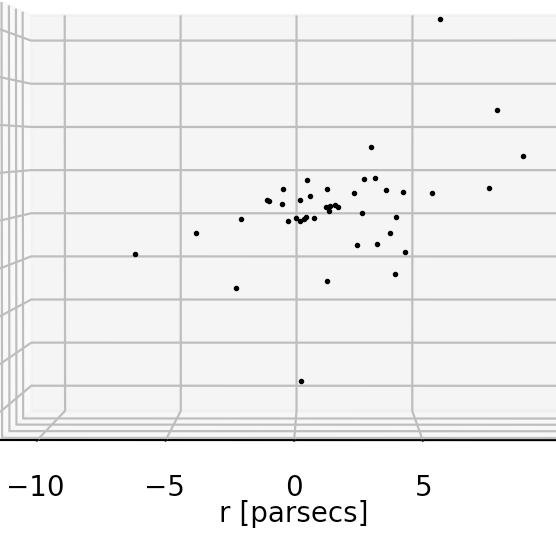
\includegraphics[width=0.4\textwidth]{Cluster.png}
    
    
    \captionof{\textbf{Figure 2.}} {\small}{Cluster simulation for $N=200$ particles, no IMBH present. Particles placed inside sphere $R=10$ parsecs }

\vspace{2mm} 
    
These initial conditions were run through a position and velocity updater, that used the leapfrog approximation. When particles come close together a very small timestep would be required to deal with the massive accelerations otherwise the particles will be ejected out of the cluster. Therefore, a softening term was introduced Eqn.\ref{F} introduced to make the particles behave, effectively, like balls of radii $\epsilon/2$, where $\epsilon$ is the softening constant.
\begin{equation}
    \textbf{F}_{i} = -G \sum^N m_i m_j \frac{\textbf{r}_i - \textbf{r}_j} {[|r_i-r_j|^2+\epsilon^2]^\frac{3}{2}}.
    \label{softened}
\end{equation}
The positions and velocities for each timestep were stored. Using the velocities and positions stored and Eqn.\ref{T} and Eqn.\ref{V}  the total kinetic and potential energy at every timestep was calculated and plotted against the cluster age. Furthermore, a velocity disperion profile was calculated as the cluster reached a "steady" state (initial collapse oscillations had calmed down, and kinetic and potential roughly constant). 

\section{Results}


\section{Discussion}


\section{Conclusion}


\subfile{Bibliography}



\end{multicols}

\end{document}
